\documentclass{article}
\usepackage{ctex}
\usepackage{amsmath}
\usepackage{amsfonts}
\usepackage{geometry}
\usepackage{graphicx}
\usepackage{listings}
\usepackage{enumerate}
\usepackage{romannum}
\usepackage{algorithm,algorithmic}
\geometry{top=2.5cm,bottom = 2.5cm, right = 2.5cm, left = 2.5cm}
\usepackage[colorlinks,linkcolor=blue,citecolor=red]{hyperref}
\usepackage[usenames,dvipsnames]{color}
\lstset{language=python,
		basicstyle=\ttfamily,
		backgroundcolor=\color{white},
		showspaces=false,
		frame=lines,
		rulecolor=\color{black},
		tabsize=2,
		captionpos=b,
		breaklines=true,
		breakatwhitespace=false,
		keywordstyle=\color{RoyalBlue},
		commentstyle=\color{YellowGreen},
		stringstyle=\color{ForestGreen}
}
\title{Estimating Riemann Curvature Tensor on Point Cloud Data in High Dimension}
\author{张翰宇{}2014012168}
\date{}
\begin{document}
\maketitle
\section{概要}
今年暑假期间,我在美国西雅图的华盛顿大学统计系进行研修. 我在Marina Meila教授的指导下,对数据流形的曲率估计这一问题进行了较为深入的研究. 在高维数据处理中,我们经常把数据点看作是在一个潜在的数据流形上进行均匀采样得到的点集. 在之前的流形学习算法,例如LLE,ISOMAP,LTSA等算法中,流形学习的主要目标都是对高维数据进行降维.然后再用我们常见的数据分析方法进行处理. 但Marina Meila教授和我的这个课题,开始关注数据流形内蕴的几何结构. 我们首先想要从数据中获得的就是这个潜在的数据流形的曲率的信息. 
黎曼曲率张量是刻画一个黎曼流形局部“弯曲程度”的重要几何量. 它是一个4阶张量,在黎曼几何中扮演着极其重要的角色. 可以说,如果能够成功地将它计算出来,我们对于这个潜在的数据结构的形状就有了基本的把握. 为此我们目前已经得到了一个可以计算任意维度$d$的黎曼流形的曲率张量的算法. 我们主要利用的是曲率张量的线性性质和Gauss-Bonnet公式,将一个点和近邻的两个数据点进行组合,进行一次估计. 在重复多次后,将曲率张量的计算问题转化成了一个优化问题. 我们将设计出来的算法在4维球面,3维平坦环面,2维环面和2维伪球面上进行了模拟实验,得到了较准确的结果. 现在这个课题进入了理论证明阶段,我们将要证明算法的渐近无偏性,并分析复杂度.
\section{Estimation Step}
The algorithm to estimate the Riemann curvature tensor can be divided into three stages:
\begin{enumerate}
	\item Construct $\varepsilon-$NN or $K-$NN neighborhood graph for the data point, Decide the intrinsic dimension of the data manifold $d$ and find bases for the tangent space $T_p\mathcal{M}$ at every point $p$ on the manifold using local Principal Component Analysis(PCA). 
	\item Choose all possible two points in the neighborhood and calculate the Gaussian curvature of this section(which is the sectional curvature) and repeat this process for $H$ times.
	\item Solve an optimization problem to find the values of every component $Rm(X,Y,Z,W)$ of the Riemann curvature tensor.
\end{enumerate}

\subsection{Local PCA for tangent space estimation}
As traditional manifold learning method works, the input data for a manifold learning algorithm is a set of point $\mathcal{D}=\{x_i\}_{i=1}^N \subset \mathcal{M} \subset \mathbb{R}^D$. We preprocess the data by first constructing a neighborhood graph $\mathcal{G}=(V,E)$ where $V$ are the vertices and $E$ the edges of $\mathcal{G}$. Here in the graph we define the neighborhood of a point $p$ as the set of points whose distance to $p$ is less than $\sqrt{\varepsilon}$. And we only connect one point with its neighbors in the graph. Note that this graph is symmetric naturally.
\par
Here we follow the standard technique that many tangent based manifold learning adopt to estimate the tangent space at every point $p$ on the manifold such as \cite{VDM} \cite{ltsa} etc. 
\par
Let us denote the number of neighboring number of $p$ by $N_p$ and the neighbors of $p$ to be $x_1,\cdots,x_{N_p}$. We always assume that $\varepsilon$ is large enough so that $N_p>d$, which is the instrinsic dimension of the underlying data manifold. But also $\varepsilon$ should be small enough that $N_i\ll N$. 
\par
Then we combine the neighborhood matrix
\begin{equation}
	X_p = [x_{i_1}-p,\cdots,x_{N_p}-p]
\end{equation}
Or we can re centralize it to the mean point of the neighborhoods. Then we construct a weight matrix $D_i$, which is an $N_i\times N_i$ diagonal matrix and
\begin{equation}
	D_p(j,j)=\sqrt{K\left(\frac{\parallel p-x_j\parallel ^2}{\sqrt{\varepsilon}}\right)}
\end{equation}
where $K(\cdot)$ is a kernel. or weight function. For example we can choose the heat kernel with $K(u)=\exp(-u^2)$. This weight allign more weights to the nearer points to $p$. Then we multiply neighborhood matrix with weight matrix and get
\begin{equation}
	B_p=X_pD_p
\end{equation}
And we can canduct a SVD decomposition of $B_p=U_p\Sigma_pV_p^T$ and get the singular values of $B_p$ by $\sigma_{p,1}\geq\sigma_{p,2}\geq\cdots$. We can write the columns of $D \times N_p$ matrix $U_p$ as
\begin{equation}
	U_p=[\boldsymbol{u}_{p_1},\boldsymbol{u}_{p_2},\cdots,\boldsymbol{u}_{p_{N_p}}]
\end{equation}
And then we take the first $d$ columns and can get our estimation of the base of the tangent space
\begin{equation}
	O_p=[\boldsymbol{u}_{p_1},\boldsymbol{u}_{p_2},\cdots,\boldsymbol{u}_{p_{d}}]
\end{equation}
And \cite{VDM} have more specific discussion of local PCA for interesting readers.

\subsection{Resampling to get sectional curvatures}
 For two points $a,b$ in the neighborhood of point $p$, we suppose that 
 $\gamma_a$ and $\gamma_b$ are the geodesics connecting $p$ to $a$ and $b$ in the manifold and $\boldsymbol{a},\boldsymbol{b}$ are the tangent vectors of $\gamma_s$ and $\gamma_t$ at point $p$. Then we can form a 2-manifold $\romannum{2}(\boldsymbol{a},\boldsymbol{b})$ as the section: the image of the exponential map of the plane in the tangent space spanned by $\{\boldsymbol{a},\boldsymbol{b}\}$. Since $\gamma_s$ and $\gamma_t$ curves locally minimizing distance from $p$ to $s$ and $t$ on the whole manifold, they should also be geodesics on $\romannum{2}(\boldsymbol{a},\boldsymbol{b})$. Then we imagine an additional geodesic connecting $s$ and $t$ on $\romannum{2}(\boldsymbol{a},\boldsymbol{b})$
\par
Now let's turn to the geodesic triangle $\Delta_{pst}$ on the 2-manifold. The Gauss-Bonnet formula will be simpler since we are considering geodesic triangle:
\begin{equation}
	 	\iint_{\Delta{pab}}KdA =\alpha_p+\alpha_a+\alpha_b - \pi
\end{equation}
Here $\alpha_p$ is the smaller angle between $\boldsymbol{a},\boldsymbol{b}$ on the tangent plane. And $\alpha_a,\alpha_b$ are similarly defined.
Therefore, we have the following approximation of the Gaussian curvature of the 2-manifold $\romannum{2}(\boldsymbol{a},\boldsymbol{b})$
\begin{equation}
	\widehat{K}(\boldsymbol{a},\boldsymbol{b})\approx\frac{\alpha_p+\alpha_a+\alpha_b-\pi}{\text{Area}(\Delta_{pab})}
	\label{approxK}
\end{equation}
at point $p$. For this apporximation we naively suppose that $K$ is almost constant on the small neighborhood of $p$ on this section plane.
\par
We know that the sectional curvature is actually related to the Riemann curvature tensor by 
\begin{equation}
	K(\boldsymbol{a},\boldsymbol{b})=\frac{Rm(\boldsymbol{a},\boldsymbol{b},\boldsymbol{b},\boldsymbol{a})}{|\boldsymbol{a}|^2|\boldsymbol{b}|^2-\langle \boldsymbol{a},\boldsymbol{b}\rangle^2}
	\label{secCurve}
\end{equation}
Therefore considering the linear expansion of $\boldsymbol{a},\boldsymbol{b}$ on the local tangent space
\begin{equation}
	\boldsymbol{a}=\sum_{i=1}^da_i\boldsymbol{u}_{pi},\quad \boldsymbol{b}=\sum_{i=1}^db_i\boldsymbol{u}_{pi}
	\label{expandst}
\end{equation}
Since it is known that the Riemann curvature tensor is multilinear over $\mathbb{R}$, we have
\begin{equation}
	Rm(\boldsymbol{a},\boldsymbol{b},\boldsymbol{b},\boldsymbol{a})=\sum_{i_1=1}^d\sum_{i_2=1}^d\sum_{i_3=1}^d\sum_{i_4=1}^da_{i_1}b_{i_2}b_{i_3}a_{i_4}Rm(\boldsymbol{u}_{i_1},\boldsymbol{u}_{i_2},\boldsymbol{u}_{i_3},\boldsymbol{u}_{i_4})
	\label{linexpan}
\end{equation}
Therefore with \ref{secCurve} and \ref{linexpan},
\begin{equation}
	K(\boldsymbol{a},\boldsymbol{b})\left(\sum_{i=1}^da_i^2\sum_{j=1}^db_j^2-(\sum_{k=1}^da_kb_k)^2\right)=\sum_{i_1=1}^d\sum_{i_2=1}^d\sum_{i_3=1}^d\sum_{i_4=1}^da_{i_1}b_{i_2}b_{i_3}a_{i_4}Rm(\boldsymbol{u}_{i_1},\boldsymbol{u}_{i_2},\boldsymbol{u}_{i_3},\boldsymbol{u}_{i_4})
	\label{Maineq}
\end{equation}
And we substitute our estimation of $K$ there, we have a linear equation for the components $R_{ijkl}=Rm(\widehat{\boldsymbol{u}}_i,\widehat{\boldsymbol{u}}_j,\widehat{\boldsymbol{u}}_k,\widehat{\boldsymbol{u}}_l)$.
\par
Now let's repeat this process for every possible combination of $(\boldsymbol{a},\boldsymbol{b})$ in neighborhood of $\boldsymbol{p}$ and satisfying that $\parallel \boldsymbol{a}-\boldsymbol{b} \parallel< \varepsilon$. We naively use the projection of $s-p,t-p$ onto the tangent space $T_p\mathcal{M}$ to approximate $\boldsymbol{a},\boldsymbol{b}$. 
\begin{equation}
	\widehat{\boldsymbol{a}}=O_p^T(s-p)=\sum_{i=1}^d\widehat{a}_i\widehat{\boldsymbol{u}}_i,\quad \widehat{\boldsymbol{b}}=O_p^T(s-p)=\sum_{i=1}^d\widehat{b}_i\widehat{\boldsymbol{u}}_i
	\label{expandabest}
\end{equation}
For the $l-$th time we get an equation
\begin{equation}
	\widehat{K}(\widehat{\boldsymbol{a}}^{l},\widehat{\boldsymbol{b}}^l)\left(\sum_{i=1}^d(\widehat{a}_i^{l})^2\sum_{j=1}^d(\widehat{b}_j^l)^2-(\sum_{k=1}^d\widehat{a}_k^l\widehat{b}_k^l)^2\right)=\sum_{i_1=1}^d\sum_{i_2=1}^d\sum_{i_3=1}^d\sum_{i_4=1}^d\widehat{a}_{i_1}^l\widehat{b}_{i_2}^l\widehat{b}_{i_3}^l\widehat{a}_{i_4}^lRm(\widehat{\boldsymbol{u}}_{i_1},\widehat{\boldsymbol{u}}_{i_2},\widehat{\boldsymbol{u}}_{i_3},\widehat{\boldsymbol{u}}_{i_4})
	\label{Mainesteq}
\end{equation}
Putting all this equation together we will have a linear system to solve for components of Riemann curvature tensor. And according to the symmetrical properties of the Riemann curvature tensor, we should add the following restrictions which hold for arbitrary combination of $(i,j,k,l)$ in $\{1,2,\cdots,d\}^4$
\begin{align}
&Rm(\widehat{\boldsymbol{u}}_i,\widehat{\boldsymbol{u}}_j,\widehat{\boldsymbol{u}}_k,\widehat{\boldsymbol{u}}_l)=-Rm(\widehat{\boldsymbol{u}}_j,\widehat{\boldsymbol{u}}_i,\widehat{\boldsymbol{u}}_k,\widehat{\boldsymbol{u}}_l)=-Rm(\widehat{\boldsymbol{u}}_i,\widehat{\boldsymbol{u}}_j,\widehat{\boldsymbol{u}}_l,\widehat{\boldsymbol{u}}_k)=Rm(\widehat{\boldsymbol{u}}_k,\widehat{\boldsymbol{u}}_l,\widehat{\boldsymbol{u}}_i,\widehat{\boldsymbol{u}}_j)\\
&Rm(\widehat{\boldsymbol{u}}_i,\widehat{\boldsymbol{u}}_j,\widehat{\boldsymbol{u}}_k,\widehat{\boldsymbol{u}}_l)+Rm(\widehat{\boldsymbol{u}}_i,\widehat{\boldsymbol{u}}_k,\widehat{\boldsymbol{u}}_l,\widehat{\boldsymbol{u}}_j)+Rm(\widehat{\boldsymbol{u}}_i,\widehat{\boldsymbol{u}}_l,\widehat{\boldsymbol{u}}_j,\widehat{\boldsymbol{u}}_k)=0
\end{align}

\subsection{Optimization to solve the linear system}
Unfortunately direct estimation and solution to the linear system cannot give a stable result. Therefore we are turning to an optimization problem to solve for our Riemann curvature tensor. Before that we introduce some notations out of simplicity. We use $\otimes$ to denote the kroecker product of matrices and vec to denote an operator which maps $n\times n$ matrix
\[
\boldsymbol{A} = 
\begin{pmatrix}
a_{11} & a_{12} & \cdots & a_{1n} \\
a_{21} & a_{22} & \cdots & a_{2n} \\
\vdots & \vdots & \vdots & \vdots \\
a_{n1} & a_{n2} & \cdots & a_{nn} \\
\end{pmatrix}
\]
into a $n^2$ vector
\begin{equation}
\text{vec}(\boldsymbol{A})=[a_{11},a_{12},\cdots,a_{1n},a_{21},a_{22},\cdots,a_{nn}]^T
\end{equation}
\par
 Let $\boldsymbol{R}$ denote a vector representing the Riemann curvature tensor. First for every fixed $i,j$ we use a $d\times d$\ matrix $(\boldsymbol{R}_{ij})_{kl}$ to denote the matrix
\begin{equation}
	\begin{pmatrix}
	Rm(\widehat{\boldsymbol{u}}_i,\widehat{\boldsymbol{u}}_j,\widehat{\boldsymbol{u}}_1,\widehat{\boldsymbol{u}}_1) & Rm(\widehat{\boldsymbol{u}}_i,\widehat{\boldsymbol{u}}_j,\widehat{\boldsymbol{u}}_1,\widehat{\boldsymbol{u}}_2) &\cdots& Rm(\widehat{\boldsymbol{u}}_i,\widehat{\boldsymbol{u}}_j,\widehat{\boldsymbol{u}}_1,\widehat{\boldsymbol{u}}_d) \\
	Rm(\widehat{\boldsymbol{u}}_i,\widehat{\boldsymbol{u}}_j,\widehat{\boldsymbol{u}}_2,\widehat{\boldsymbol{u}}_1) & Rm(\widehat{\boldsymbol{u}}_i,\widehat{\boldsymbol{u}}_j,\widehat{\boldsymbol{u}}_2,\widehat{\boldsymbol{u}}_2) &\cdots &Rm(\widehat{\boldsymbol{u}}_i,\widehat{\boldsymbol{u}}_j,\widehat{\boldsymbol{u}}_2,\widehat{\boldsymbol{u}}_d) \\
	\vdots & \vdots & \vdots & \vdots \\
	Rm(\widehat{\boldsymbol{u}}_i,\widehat{\boldsymbol{u}}_j,\widehat{\boldsymbol{u}}_d,\widehat{\boldsymbol{u}}_1) & Rm(\widehat{\boldsymbol{u}}_i,\widehat{\boldsymbol{u}}_j,\widehat{\boldsymbol{u}}_d,\widehat{\boldsymbol{u}}_2) &\cdots& Rm(\widehat{\boldsymbol{u}}_i,\widehat{\boldsymbol{u}}_j,\widehat{\boldsymbol{u}}_d,\widehat{\boldsymbol{u}}_d) \\
	\end{pmatrix}
\end{equation}
Then we put all these $\boldsymbol{R}_{ij}$ together as a $d^2\times d^2 $\ block matrix
\begin{equation}
	\widetilde{\boldsymbol{Rm}}=
	\begin{pmatrix}
	\boldsymbol{R}_{11} & \boldsymbol{R}_{12}&\cdots &\boldsymbol{R}_{1d} \\
	\boldsymbol{R}_{21} & \boldsymbol{R}_{22}&\cdots &\boldsymbol{R}_{2d} \\
	\vdots & \vdots & \vdots & \vdots \\
	\boldsymbol{R}_{d1} & \boldsymbol{R}_{d2}&\cdots& \boldsymbol{R}_{dd} \\
	\end{pmatrix}
\end{equation}
And finally we construct our vector $\boldsymbol{Rm}=\text{vec}(\widetilde{\boldsymbol{Rm}})$. We will use $R_{ijkl}$ to denote the $kl-$ element in the matrix $\boldsymbol{R}_{ij}$, which is $Rm(\widehat{\boldsymbol{u}}_i,\widehat{\boldsymbol{u}}_j,\widehat{\boldsymbol{u}}_k,\widehat{\boldsymbol{u}}_l)$ 
\par
Then rewrite \ref{Mainesteq} we can get a loss function

\begin{equation}
	E_d(l)= \left(\widehat{K}(\widehat{\boldsymbol{a}}^l,\widehat{\boldsymbol{b}}^l)-\frac{(\widehat{\boldsymbol{a}}^l\otimes(\widehat{\boldsymbol{b}}^l\otimes(\widehat{\boldsymbol{b}}^l\otimes\widehat{\boldsymbol{a}}^l)))^T\boldsymbol{Rm}}{|\widehat{\boldsymbol{a}}^l|^2|\widehat{\boldsymbol{b}}^l|^2-|\langle \widehat{\boldsymbol{a}}^l,\widehat{\boldsymbol{b}}^l\rangle|^2}\right)^2
	\label{loss}
\end{equation}
Therefore our goal is to solve the linear system by considering the following optimization problem since directly solving for the system may be very unstable numerically.
\begin{align}
\notag
\textbf{min}\quad &\rho(E(l)) \\
\notag
\mathbf{s.t.}\quad &R_{ijkl}=-R_{jikl}=-R_{ijlk}=R_{klij} \\
& R_{ijkl}+R_{iklj}+R_{iljk} = 0
\label{problem}
\end{align}
Here $\rho$ can be choosed as Huber loss to get a stable result.
\begin{equation}
	\rho(u)=\begin{cases}u^2,&\quad |u|\leq M\\ M(2|u|-M),&\quad |u|>M \end{cases}
\end{equation}
It is not easy to solve this constrained optimization problem \ref{problem}
However, fortunately all the constraints are linear equality constraints. And we are able to only look for the independent components of the Riemann curvature tensor as another vector $\boldsymbol{R}$. Then we can construct a stretching matrix $\boldsymbol{S}$ and multiply it to the left of $\boldsymbol{R}$ to get $\boldsymbol{Rm}$. Here we give an example of how to construct $\boldsymbol{R}$ and $\boldsymbol{S}$.
\par
The independent components in Riemann curvature tensor including several cases:
\begin{enumerate}[(a)]
	\item For every $i \in \{1,2,\cdots,d\}, R_{iiii}=0$, therefore they are not needed in $\boldsymbol{R}$.
	\item There are two different indexes in $(i,j,k,l)$, the only independent and nonzero component is $R_{ijij}$. There are $\binom{d}{2}=d(d-1)/2$ of them. 
	\item There are three different indexes in $(i,j,k,l)$, we assume that depending on which number (minimum, median, maximum) is the repeated index, there are three independent values. Totally there are $3\binom{d}{3}=d(d-1)(d-2)/2$ of them.
	\item Four indexes are all different, let $\sigma(\cdot)$ representing the ascending order index of $\cdot$ in the four indexes, then we can divide them into three subgroups: 
	\begin{enumerate}[i)]
		\item $|\sigma(i)-\sigma(j)|=|\sigma(k)-\sigma(l)|=1$
		\item $|\sigma(i)-\sigma(j)|=|\sigma(k)-\sigma(l)|=2$
		\item $|\sigma(i)-\sigma(j)|\neq|\sigma(l)-\sigma(k)|$
	\end{enumerate}
	And when we know two values of $R_{ijkl}$ falling in two of the three cases, we can have all values of components with permutations of $\{i,j,k,l\}$. All the independent components add up to $\frac{2}{3}\frac{d(d-1)(d-2)(d-3)}{8}$
\end{enumerate}
Therefore we have $\frac{1}{12}d^2(d^2-1)$ independent components of Riemann curvature tensor in total. We will use the following notations:
\begin{align*}
f_2(i,j)\quad \quad & =\sum_{i_1=1}^{i-1}(d-i_1)+(j-i)=\frac{1}{2}(2d-i)(i-1)+(j-i)\quad(i<j) \\
f_3(i,j,k)\quad &= \sum_{i_1=1}^{i-1}\sum_{i_2=i_1+1}^{d-1}(d-i_2)+\sum_{i_2=i+1}^{j-1}(d-i_2)+(k-j) \\ &=\frac{1}{6} \left(3 d^2 i-3 d^2-3 d i^2+3 d+i^3-i\right)-\frac{1}{2} (i-j+1) (2
    d-i-j)-j+k \\
f_4(i,j,k,l) & = \sum_{i_1=1}^{i-1}\sum_{i_2=i_1+1}^{d-2}\sum_{i_3=i_2+1}^{d-1}(d-i_3) + \sum_{i_2=i+1}^{j-1}\sum_{i_3=i_2+1}^{d-1}(d-i_3)+\sum_{i_3=j+1}^{d-1}(d-i_3)+(l-k) \\ &=-\frac{1}{6} (i-j+1) \left(3 d^2-3 d i-3 d j-3 d+i^2+i j+2 i+j^2+j\right)-\frac{1}{2} (j-k+1) (2 d-j-k)-k+l\\&+\frac{1}{24}
   \left(4 d^3 i-4 d^3-6 d^2 i^2-6 d^2 i+12 d^2+4 d i^3+6 d i^2-2 d i-8 d-i^4-2 i^3+i^2+2
   i\right)\\
\end{align*}
Then we briefly state our construction of $\boldsymbol{R}$ as following (we always suppose $i<j<k<l$):
\begin{align}
\notag
&\boldsymbol{R}_{f_2(i,j)}=R_{ijij} \\
\notag
&\boldsymbol{R}_{\binom{d}{2}+3(f_3(i,j,k)-1)+1} = R_{ijki} \\
\notag
&\boldsymbol{R}_{\binom{d}{2}+3(f_3(i,j,k)-1)+2} = R_{jikj} \\
\notag
&\boldsymbol{R}_{\binom{d}{2}+3(f_3(i,j,k)-1)+3} = R_{kijk} \\
\notag
&\boldsymbol{R}_{\binom{d}{2}+3\binom{d}{3}+2(f_4(i,j,k,l)-1)+1} = R_{ijkl}\\
&\boldsymbol{R}_{\binom{d}{2}+3\binom{d}{3}+2(f_4(i,j,k,l)-1)+2} = R_{ikjl}
\end{align}
And then for each row in the stretching matrix $\boldsymbol{S}$, we assign one or two elements to 1 or -1 according to the symmetric properties and bianchi identities. For example with the case $d=2$ we have only 1 independent component in the riemann curvature tensor, so we have 
\begin{equation}
	\boldsymbol{R}=R_{1212},\boldsymbol{S}=[0,0,0,0,0,1,-1,0,0,-1,1,0,0,0,0,0]^T
\end{equation}
And then the problem \ref{problem} can be transfered into a non constraint optimization problem with a newly defined loss function
\begin{equation}
	E_d(l)= \left(\widehat{K}(\widehat{\boldsymbol{a}}^l,\widehat{\boldsymbol{b}}^l)-\frac{(\widehat{\boldsymbol{a}}^l\otimes(\widehat{\boldsymbol{b}}^l\otimes(\widehat{\boldsymbol{b}}^l\otimes\widehat{\boldsymbol{a}}^l)))^T\boldsymbol{S}\boldsymbol{R}}{|\widehat{\boldsymbol{a}}^l|^2|\widehat{\boldsymbol{b}}^l|^2-|\langle \widehat{\boldsymbol{a}}^l,\widehat{\boldsymbol{b}}^l\rangle|^2}\right)^2
	\label{loss2}
\end{equation}
and we want to find the $\boldsymbol{R}$ in $\mathbb{R}^{(d(d-1)/12)}$ that minimize the loss function $E(l)$. Such optimization problems are actually not easy to solve this optimization problem but at least we could use iterative reweighted least squares algorithm to find the solution.
\par
Let's look at a special case in  2-dimension surfaces. In this scenario, the tangent space also has dimension 2. Therefore the Gaussian curvature is the same no matter how the two neighbor data points are chosen. Let $\boldsymbol{u}_1,\boldsymbol{u}_2$ be the orthonormal base of $T_p\mathcal{M}$ at point $p$, then we randomly choose $a^l,b^l$ in the neighborhood of $p$, then \ref{expandabest} could be reduced to 
\begin{equation}
	\widehat{\boldsymbol{a}}^l=\widehat{a}_1\widehat{\boldsymbol{u}}_1+\widehat{a}_2\widehat{\boldsymbol{u}}_2,\quad \widehat{\boldsymbol{b}}=\widehat{b}_1\widehat{\boldsymbol{u}}_1+\widehat{b}_2\widehat{\boldsymbol{u}}_2
\end{equation}
Then we con have the $2^4=16-$vector
\begin{equation}
	\widehat{\boldsymbol{a}^l}\otimes(\widehat{\boldsymbol{b}^l}\otimes\widehat{(\boldsymbol{b}^l}\otimes\widehat{\boldsymbol{a}^l}))=[\widehat{a}_1\widehat{b}_1\widehat{b}_1\widehat{a}_1,\widehat{a}_1\widehat{b}_1\widehat{b}_1\widehat{a}_2,\widehat{a}_1\widehat{b}_1\widehat{b}_2\widehat{a}_1,\cdots,\widehat{a}_2\widehat{b}_2\widehat{b}_2\widehat{a}_2]
\end{equation}
Combining with our stretching matrix $S$ we can rewrite the loss function as

\begin{align}
	\notag
	E_2(l)&=\left(\widehat{K}(\widehat{\boldsymbol{a}}^l,\widehat{\boldsymbol{b}}^l)-\frac{(\widehat{\boldsymbol{a}}^l\otimes(\widehat{\boldsymbol{b}}^l\otimes(\widehat{\boldsymbol{b}}^l\otimes\widehat{\boldsymbol{a}}^l)))^T\boldsymbol{S}\boldsymbol{R}}{|\widehat{\boldsymbol{a}}^l|^2|\widehat{\boldsymbol{b}}^l|^2-|\langle \widehat{\boldsymbol{a}}^l,\widehat{\boldsymbol{b}}^l\rangle|^2}\right)^2 \\
	\notag
	&=\left(\widehat{K}(\widehat{\boldsymbol{a}}^l,\widehat{\boldsymbol{b}}^l)+\frac{(\widehat{a}_1^l\widehat{b}_2^l-\widehat{a}_2^l\widehat{b}_1^l)^2R_{1212}}{(\widehat{a}_2^l\widehat{b}_1^l-\widehat{a}_1^l\widehat{b}_2^l)^2}\right)^2 \\
	&=\left(\widehat{K}(\widehat{\boldsymbol{a}}^l,\widehat{\boldsymbol{b}}^l)+R_{1212}\right)^2 
\end{align}
We can see that in the case of $2-$dimensions our optimization problem will degenerate to find value that minimizes the negative of the estimated Gaussian curvature.
\par
Now we can summarize our estimation step into a curvature estimation algorithm
\begin{algorithm}
	\renewcommand{\algorithmicrequire}{\textbf{Input:}}
	\renewcommand{\algorithmicensure}{\textbf{Output:}}
	\caption{Curvature Tensor Estimation}
	\begin{algorithmic}[1]
	\REQUIRE $N$ data points in dimension $D$ $\{x_i\}_{i=1}^N$, a point $p$ that we want to estimated the curvature tensor
	\ENSURE The coefficients of Riemann curvature tensor at point $p$
	\STATE Construct the $\varepsilon-$neighbor graph $\mathcal{G}$ and the weight matrix $W$ using the heat kernel
	\STATE Conduct local PCA algorithm to estimate local tangent space at $p$ and all neighbors of $p$
	\FOR{every pair of $(a,b)$ in the neighborhood of $p$}
		 \IF{$b$ is in the neighborhood of $a$}
		 	\STATE Estimate the gaussian curvature using Gauss-Bonnet formula
		 \ENDIF
	\ENDFOR
	\STATE Minimizing loss function \ref{loss2} to get the estimation.
	\end{algorithmic}
\end{algorithm}
\section{Simulation}
In this section results of some numeric simulation experiments are reported. We tested our algorithm on the following four models:
\begin{itemize}
	\item 4-dimension sphere $\mathbb{S}^4$ embedded in 5 dimension Eulidean space.
	\item 3-dimension flat torus $\mathbb{T}^3$ embedded in 4 dimension Euclidean space.
	\item 2-dimension curved torus embedded in 3 dimension space
	\item 2-dimension pseudosphere embedded in 2 dimension space
\end{itemize}
For every model, we fixed the sample size 20000, and sampled uniformly distributed on it (specified later). Then we choose epsilon such that for each point the average number of neighbors is approximately $10^2$. We randomly choose one point a time in every model, calculate the Riemann curvature there as we proposed and then repeat the whole process for 10000 times. The results are evaluated (specified later) basically by the mean absolute value of the Frobenius norm of our estimated $\widehat{\boldsymbol{R}}$ and the true value $\boldsymbol{R}$
\\
\par
\textbf{4d-Sphere in $\mathbb{R}^5$} The data is sampled as \cite{Uniform}, we generate 4-dimension standard normal distribution random numbers and then normalise them to get uniform distributed data. The true value of Riemann curvature tensor of a 4d-sphere with radius $R$ is
\begin{equation}
	R_{ijkl}=\frac{1}{R^2}(g_{il}g_{jk}-g_{ik}g_{jl})
\end{equation}
for any basis. Therefore with $R=1$,the true value of $\boldsymbol{R}$ is
\begin{equation}
	\boldsymbol{R}=(\overbrace{-1,-1,\cdots,-1}^{6},\overbrace{0,0,\cdots,0}^{10})
\end{equation} In case that the average number of neighbors for every point is approximately 100, we choose $\epsilon=0.40$
Then the distribution of repeated result of estimation can be shown in figures. 
\begin{figure}[htbp]
\centering
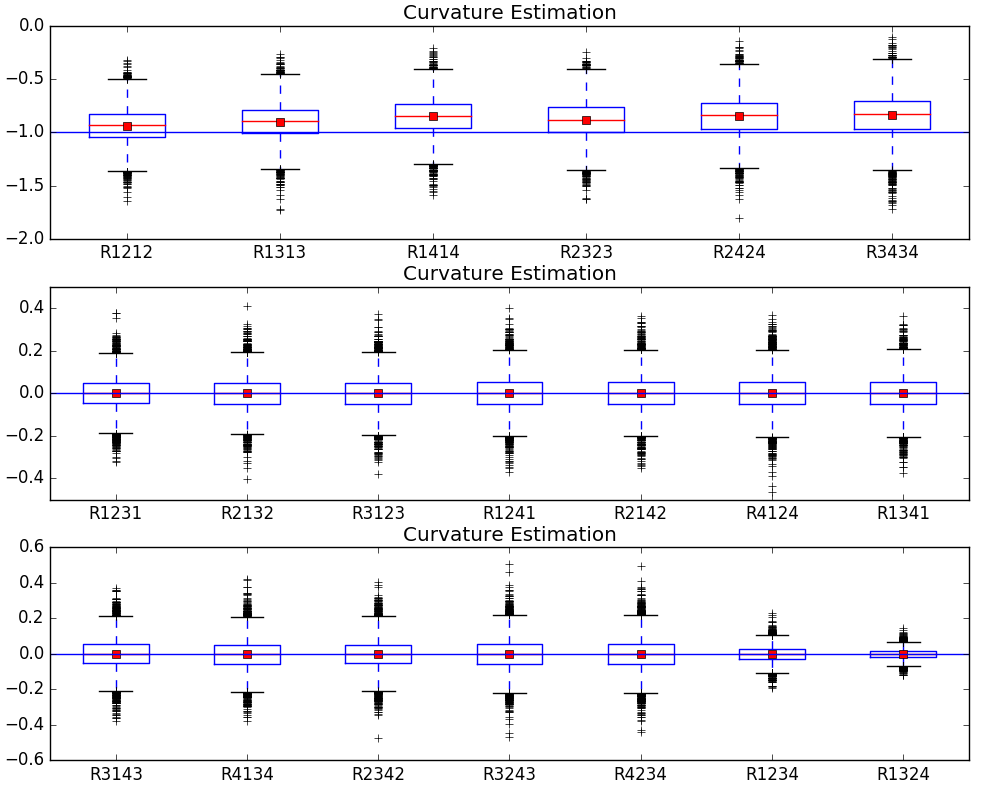
\includegraphics[width=0.8\textwidth]{sphere4d.png}
\end{figure}

\par
\textbf{3d-Flat torus in $\mathbb{R}^4$} Here the 3d-flat torus is given by the parametrization
\begin{equation}
	(\cos u,\sin u,\cos v,\sin v, \cos w,\sin w),\quad u,v,w\in[0,2\pi)
\end{equation}
And the true value for every component is 0 according to standard calculation of Riemann curvature tensor. The data is sampled uniformly by first finding uniformly distributed sample on three perpendicular $\mathbb{S}^1$ circles and then generate there cartesian product.In our simulation, we select $R=2,r=1$. We choose epsilon = $0.63$ to guarantee approximately 100 neighbors in average for every point. The true value of curvature tensor for flat torus is zero for every component. The estimation results are shown in figures.
\begin{figure}[htbp]
\centering
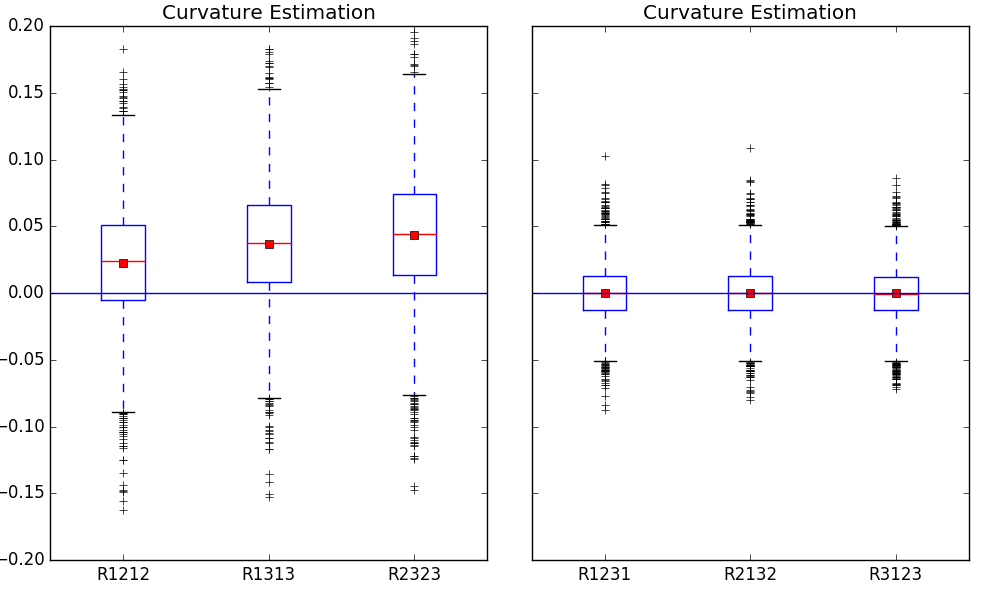
\includegraphics[width=0.8\textwidth]{torus.png}
\end{figure}
\\
\par
\textbf{2d-curved torus in $\mathbb{R}^3$} Here we test our algorithm on varying sectional curvature case. The curved torus is given by the parametrization
\begin{equation}
	((R+r\cos \theta)\cos\phi, (R+r\cos \theta)\sin\phi,r\sin\theta),\quad 0\leq \theta,\phi \leq 2\pi
\end{equation}
Sampling is conducted as \cite{Sample} Example 1A. At point $(\theta,\phi)$, since it is only two dimensional, the only one independent component of the curvature tensor is $R_{1212}=-\frac{\cos \theta}{R+r\cos \theta}$. Then we can see the estimated result as
\begin{figure}[htbp]
\centering
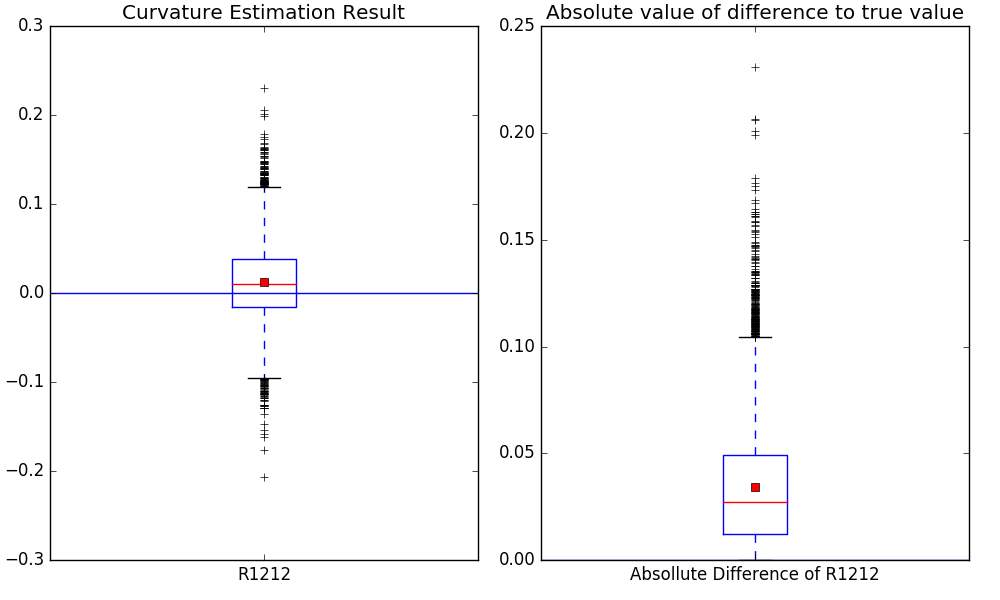
\includegraphics[width=0.8\textwidth]{ctorus.png}
\end{figure}

\par
\textbf{2d-pseudosphere in $\mathbb{R}^3$} Pseusosphere is one representative of negative constant gaussian curvature, given by the parametrization
\begin{equation}
	(\cos u \sin v, \sin u\sin v, \cos u+\log(\tan(\frac{v}{2}))),\quad u\in[0,2\pi), v\in [0,\pi)
\end{equation}
We choose $\epsilon = 0.2$ to have a proper number of average neighbors. The results are shown as
\begin{figure}[htbp]
\centering
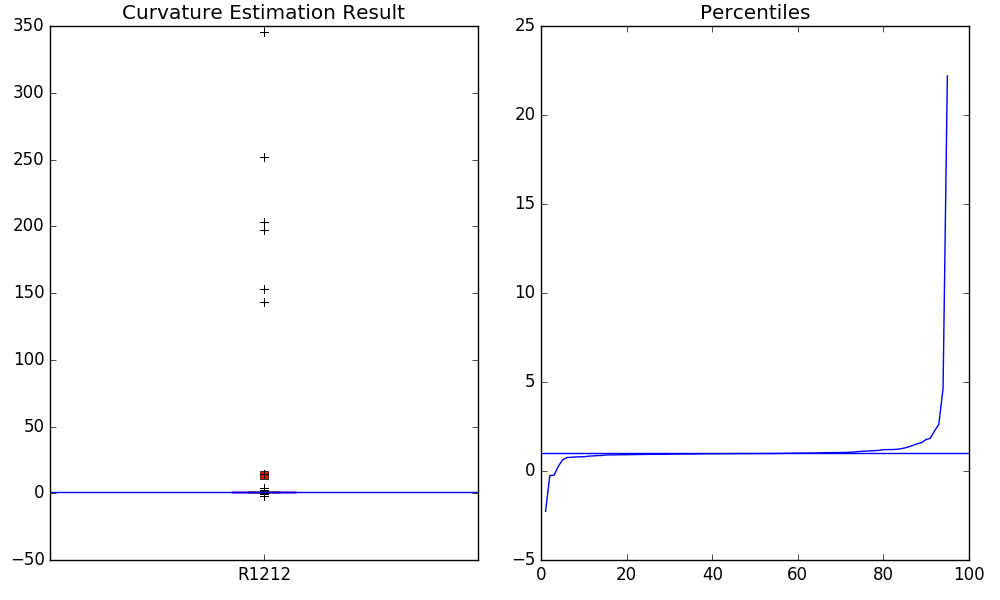
\includegraphics[width=0.8\textwidth]{psphere.png}
\end{figure}
\bibliography{curve}
\bibliographystyle{plain}
\end{document}